\chapter{Virittävät puut}

\section{Union-find-rakenne}

Union-find-rakenne pitää yllä alkioiden joukkoja ja tarjoaa
seuraavat tehokkaat operaatiot:

\begin{itemize}
\item yhdistä kaksi joukkoa samaksi joukoksi
\item tarkista, ovatko kaksi alkiota samassa joukossa
\end{itemize}

Tarkastellaan esimerkkinä tilannetta, jossa joukot ovat
$A=\{1,4\}$, $B=\{2,5,6\}$ ja $C=\{3,7,8\}$.
Tällä hetkellä alkiot $1$ ja $2$ ovat eri joukoissa.
Yhdistämme sitten joukot $A$ ja $B$,
jolloin niistä syntyy joukko $\{1,2,4,5,6\}$.
Tämän jälkeen alkiot $1$ ja $2$ ovat samassa joukossa.

Verkkojen tapauksessa voimme tulkita operaatiot näin:

\begin{itemize}
\item lisää kaari kahden erillisen komponentin välille
\item tarkista, ovatko kaksi solmua samassa komponentissa
\end{itemize}

\begin{figure}
\center
\begin{center}
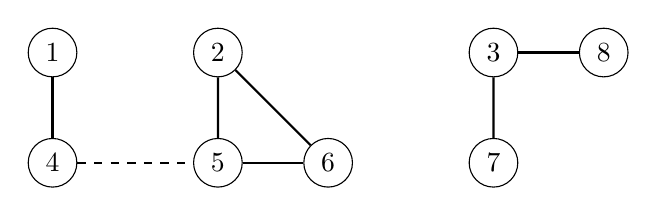
\begin{tikzpicture}[scale=0.7]
\node[draw, circle] (1) at (0,0) {$1$};
\node[draw, circle] (4) at (0,-2) {$4$};

\node[draw, circle] (2) at (3,0) {$2$};
\node[draw, circle] (5) at (3,-2) {$5$};
\node[draw, circle] (6) at (5,-2) {$6$};

\node[draw, circle] (3) at (8,0) {$3$};
\node[draw, circle] (7) at (8,-2) {$7$};
\node[draw, circle] (8) at (10,0) {$8$};

\path[draw,thick,-] (1) -- (4);
\path[draw,thick,-] (2) -- (5);
\path[draw,thick,-] (2) -- (6);
\path[draw,thick,-] (5) -- (6);
\path[draw,thick,-] (3) -- (7);
\path[draw,thick,-] (3) -- (8);

\path[draw,thick,-,dashed] (4) -- (5);
\end{tikzpicture}
\end{center}
\caption{Verkon komponentit ovat $\{1,4\}$, $\{2,5,6\}$ ja $\{3,7,8\}$.
Kun lisäämme kaaren $4-5$, kaksi komponenttia yhdistyy.}
\label{fig:veryhd}
\end{figure}

Kuvassa \ref{fig:veryhd} on äskeistä esimerkkiä vastaava tilanne verkkona.
Kun li\-säämme kaaren solmujen $4$ ja $5$ välille,
kaksi komponenttia yhdistyy ja solmut $1$ ja $2$
ovat samassa komponentissa.

\subsection{Rakenteen toteutus}

Toteutamme union-find-rakenteen niin, että jokaisessa joukossa
yksi alkioista on joukon \emph{edustaja} ja muut alkiot viittaavat
edustajaan suoraan tai muiden alkioiden kautta.
Kun haluamme tarkastaa, ovatko kaksi alkiota samassa joukossa,
selvitämme niiden edustajat ja vertaamme niitä toisiinsa.

Jokaisella joukon alkiolla $x$ on arvo $\texttt{next}[x]$,
joka kertoo seuraavan alkion viittauksien ketjussa.
Jos $\texttt{next}[x]=x$, alkio on joukon edustaja.
Tämän ansiosta saamme selville mille tahansa alkiolle $x$,
mikä on vastaavan joukon edustaja, kulkemalla läpi viittausten ketjun.

\begin{figure}
\center
\begin{center}
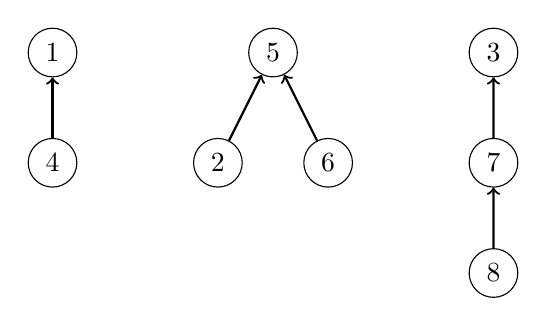
\begin{tikzpicture}[scale=0.7]
\node[draw, circle] (1) at (0,0) {$1$};
\node[draw, circle] (4) at (0,-2) {$4$};

\node[draw, circle] (2) at (3,-2) {$2$};
\node[draw, circle] (5) at (4,0) {$5$};
\node[draw, circle] (6) at (5,-2) {$6$};

\node[draw, circle] (3) at (8,0) {$3$};
\node[draw, circle] (7) at (8,-2) {$7$};
\node[draw, circle] (8) at (8,-4) {$8$};

\path[draw,thick,->] (4) -- (1);
\path[draw,thick,->] (2) -- (5);
\path[draw,thick,->] (6) -- (5);
\path[draw,thick,->] (7) -- (3);
\path[draw,thick,->] (8) -- (7);
\end{tikzpicture}
\end{center}
\caption{Union-find-rakenne, joka vastaa joukkoja $\{1,4\}$, $\{2,5,6\}$ ja $\{3,7,8\}$.}
\label{fig:unifin}
\end{figure}

Kuvassa \ref{fig:unifin} on esimerkki union-find-rakenteesta, kun joukot ovat
$A=\{1,4\}$, $B=\{2,5,6\}$ ja $C=\{3,7,8\}$.
Joukkojen edustajat ovat 1, 5 ja 3.
Esimerkiksi $\texttt{next}[1]=1$ ja $\texttt{next}[2]=5$.
Saamme selville alkion 8 joukon edustajan kulkemalla ketjua
$8 \rightarrow 7 \rightarrow 3$.

Seuraava operaatio \texttt{find} selvittää alkion $x$ joukon edustajan:

\begin{code}
int find(int x) {
    while (x != next[x]) {
        x = next[x];
    }
    return x;
}
\end{code}

Tämän avulla voimme luoda operaation \texttt{same}, joka tarkastaa,
ovatko alkiot $a$ ja $b$ samassa joukossa.
Alkiot ovat samassa joukossa täsmälleen silloin, kun niillä
on sama edustaja:

\begin{code}
boolean same(int a, int b) {
    return find(a) == find(b);
}
\end{code}

Viimeinen tarvittava operaatio on \texttt{union}, joka yhdistää alkioita
$a$ ja $b$ vastaavat joukot.
Yksinkertainen tapa toteuttaa operaatio on seuraava:

\begin{code}
void union(int a, int b) {
    a = find(a);
    b = find(b);
    next[a] = b;
}
\end{code}

Tässä toteutuksessa selvitämme ensin kummankin joukon edustajat,
ja sitten asetamme ensimmäisen edustajan viittaamaan toiseen.

Tässä kuvattu tapa toteuttaa union-find-rakenne on toimiva,
mutta se \emph{ei} ole tehokas.
Ongelmana on, että \texttt{union}-operaatiot saattavat tuottaa
pitkän viittausten ketjun, jolloin \texttt{find}- ja
\texttt{same}-operaatiot toimivat hitaasti.
Pahimmassa tapauksessa kaikki $n$ alkiota voivat olla
samassa ketjussa, jolloin operaatiot vievät aikaa $O(n)$.
Seuraavaksi toteutammekin rakenteen paremmin niin,
että pitkiä ketjuja ei pääse syntymään.

\subsection{Tehokas yhdistäminen}

Osoittautuu, että saamme aikaan tehokkaan union-find-rakenteen,
kunhan toteutamme kahden joukon yhdistämisen niin,
että asetamme \emph{pienemmän} joukon edustajan viittaamaan
\emph{suuremman} joukon edustajaan. Jos joukot ovat yhtä suuria,
voimme valita kummin vain.

\begin{figure}
\center
\begin{center}
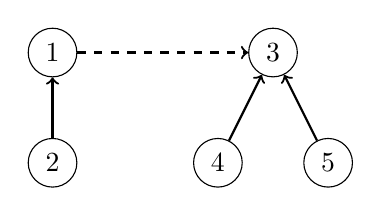
\begin{tikzpicture}[scale=0.7]
\node[draw, circle] (1) at (0,0) {$1$};
\node[draw, circle] (2) at (0,-2) {$2$};
\node[draw, circle] (3) at (4,0) {$3$};
\node[draw, circle] (4) at (3,-2) {$4$};
\node[draw, circle] (5) at (5,-2) {$5$};
\path[draw,thick,->] (2) -- (1);
\path[draw,thick,->] (4) -- (3);
\path[draw,thick,->] (5) -- (3);
\path[draw,thick,->,dashed] (1) -- (3);
\end{tikzpicture}
\end{center}
\caption{Tehokas yhdistäminen. Alkion $1$ joukon koko on 2
ja alkion $3$ joukon koko on 3,
joten yhdistämme alkion 1 alkioon 3.}
\label{fig:tehyhd}
\end{figure}


Tätä varten pidämme jokaiselle alkiolle $x$ yllä tietoa
$\texttt{size}[x]$: jos alkio $x$ on joukon edustaja,
kuinka monta alkiota joukossa on.
Kuvassa \ref{fig:tehyhd} on esimerkki tilanteesta,
jossa haluamme yhdistää alkioiden $1$ ja $3$ edustamat joukot.
Koska $\texttt{size}[1]=2$ ja $\texttt{size}[3]=3$,
asetamme viittauksen alkiosta 1 alkioon 3.
Tämän seurauksena $\texttt{size}[3]=5$.

Voimme käytännössä toteuttaa joukkojen yhdistämisen näin:

\begin{code}
void union(int a, int b) {
    a = find(a);
    b = find(b);
    if (size[a] < size[b]) {
        next[a] = b;
        size[b] += size[a];
    } else {
        next[b] = a;
        size[a] += size[b];
    }
}
\end{code}

Koodissa on kaksi tapausta sen mukaan, kumpi joukoista on suurempi.
Kummassakin tapauksessa asetamme pienemmän joukon edustajan
osoittamaan suuremman joukon edustajaan ja päivitämme suuremman
joukon koon.

Joukkojen yhdistäminen tällä tavalla takaa, että jokaisessa
viittausten ketjussa on enintään $O(\log n)$ askelta,
eli operaatiot \texttt{find} ja \texttt{same} toimivat
ajassa $O(\log n)$ ja operaatio \texttt{union} toimii ajassa $O(1)$.

Miksi sitten ketjussa on enintään $O(\log n)$ askelta?
Aina kun yhdistämme kaksi joukkoa ja lisäämme viittauksen,
pienemmän joukon koko ainakin kaksinkertaistuu viittausta kulkemalla.
Niinpä jos polulla on $k$ askelta, se johtaa joukkoon,
jossa on ainakin $2^k$ alkiota, eli jos joukossa on enintään $n$
alkiota, polun pituus on enintään $O(\log n)$ askelta.

\subsection{Polkujen tiivistäminen}

Pystymme saamaan union-find-rakenteen vielä tehokkaammaksi
toteuttamalla \texttt{find}-operaation seuraavasti:

\begin{code}
int find(int x) {
    return next[x] = find(x);
}
\end{code}

Tässä ideana on \emph{tiivistää} polkuja niin,
että aina kun kuljemme polkua pitkin, asetamme samalla
jokaisen polun alkion \texttt{next}-arvoksi niiden edustajan.
Tämän ansiosta jos kuljemme samaa polkua myöhemmin, 
pääsemme suoraan edustajaan.

\begin{figure}
\center
\begin{center}
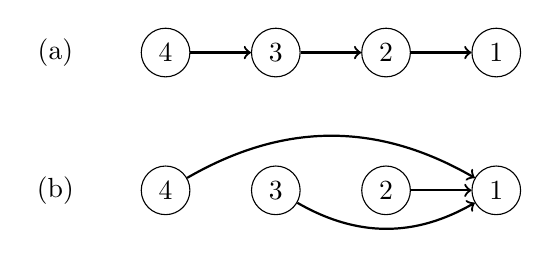
\begin{tikzpicture}[scale=0.7]
\begin{scope}
\node[draw, circle] (1) at (0,0) {$1$};
\node[draw, circle] (2) at (-2,0) {$2$};
\node[draw, circle] (3) at (-4,0) {$3$};
\node[draw, circle] (4) at (-6,0) {$4$};
\path[draw,thick,->] (4) -- (3);
\path[draw,thick,->] (3) -- (2);
\path[draw,thick,->] (2) -- (1);
\node at (-8,0) {(a)};
\end{scope}
\begin{scope}[yshift=-2.5cm]
\node[draw, circle] (1) at (0,0) {$1$};
\node[draw, circle] (2) at (-2,0) {$2$};
\node[draw, circle] (3) at (-4,0) {$3$};
\node[draw, circle] (4) at (-6,0) {$4$};
\path[draw,thick,->] (4) edge [bend left] (1);
\path[draw,thick,->] (3) edge [bend right] (1);
\path[draw,thick,->] (2) -- (1);
\node at (-8,0) {(b)};
\end{scope}
\end{tikzpicture}
\end{center}
\caption{Polun tiivistäminen. (a) Alkuperäinen polku $4 \rightarrow 3 \rightarrow 2 \rightarrow 1$.
(b) Tiivistetty polku, jossa kaikki alkiot viittaavat suoraan edustajaan.}
\label{fig:poltii}
\end{figure}

Kuva \ref{fig:poltii} näyttää esimerkin polun tiivistämisestä.
Kuljemme aluksi polkua $4 \rightarrow 3 \rightarrow 2 \rightarrow 1$,
jolloin kaikki alkiot asetetaan viittaamaan edustajaan $1$.
Seuraavan kerran pääsemme suoraan alkiosta $4$ edustajaan $1$.

On mahdollista osoittaa, että polkujen tiivistämisen ansiosta
$\texttt{find}$-ope\-raatiot vievät keskimäärin aikaa vain
$O(\alpha(n))$, missä $\alpha(n)$ on hyvin hitaasti kasvava
käänteinen Ackermannin funktio.
Tämä tarkoittaa käytännössä, että rakenteen operaatiot
ovat vakioaikaisia.
Tämän tuloksen osoittaminen on kuitenkin vaikeaa,
emmekä käsittele asiaa tällä kurssilla.

\section{Esimerkki: Kaupungit}

Maassa on $n$ kaupunkia, joiden välillä ei ole vielä yhtään tietä.
Sitten teitä aletaan rakentaa yksi kerrallaan, yhteensä $m$ tietä.
Jokainen tie on kaksisuuntainen ja yhdistää kaksi kaupunkia.
Minkä tien rakentamisen jälkeen kaikki kaupungit ovat ensimmäistä
kertaa yhteydessä toisiinsa?

\begin{figure}
\center
\begin{center}
\begin{tikzpicture}[scale=0.7,label distance=-1.5mm]
\small
\newcommand\verkko[6]{
\node[draw, circle] (1) at (0,-1) {$1$};
\node[draw, circle] (2) at (2,0) {$2$};
\node[draw, circle] (3) at (2,-2) {$3$};
\node[draw, circle] (4) at (4,0) {$4$};
\node[draw, circle] (5) at (4,-2) {$5$};
\node at (2,-3.5) {vaihe #1};
}
\begin{scope}
\verkko{1}{0}{\infty}{\infty}{\infty}{\infty}
\path[draw,thick,-] (1) -- (2);
\end{scope}
\begin{scope}[xshift=6.5cm]
\verkko{2}{0}{8}{\infty}{\infty}{\infty}
\path[draw,thick,-] (1) -- (2);
\path[draw,thick,-] (1) -- (3);
\end{scope}
\begin{scope}[xshift=13cm]
\verkko{3}{0}{8}{2}{\infty}{\infty}
\path[draw,thick,-] (1) -- (2);
\path[draw,thick,-] (1) -- (3);
\path[draw,thick,-] (2) -- (3);
\end{scope}
\begin{scope}[yshift=-5.5cm]
\verkko{4}{0}{8}{2}{13}{\infty}
\path[draw,thick,-] (1) -- (2);
\path[draw,thick,-] (1) -- (3);
\path[draw,thick,-] (2) -- (3);
\path[draw,thick,-] (4) -- (5);
\end{scope}
\begin{scope}[yshift=-5.5cm,xshift=6.5cm]
\verkko{5}{0}{6}{2}{13}{\infty}
\path[draw,thick,-] (1) -- (2);
\path[draw,thick,-] (1) -- (3);
\path[draw,thick,-] (2) -- (3);
\path[draw,thick,-] (4) -- (5);
\path[draw,thick,-] (2) -- (4);
\end{scope}
\begin{scope}[yshift=-5.5cm,xshift=13cm]
\verkko{6}{0}{6}{2}{13}{9}
\path[draw,thick,-] (1) -- (2);
\path[draw,thick,-] (1) -- (3);
\path[draw,thick,-] (2) -- (3);
\path[draw,thick,-] (4) -- (5);
\path[draw,thick,-] (2) -- (4);
\path[draw,thick,-] (2) -- (5);
\end{scope}
\end{tikzpicture}
\end{center}
\caption{Esimerkki kaupunkien yhdistämisestä teillä. Vaiheen 5 jälkeen
kaikki kaupungit ovat yhteydessä toisiinsa.}
\label{fig:kauesi}
\end{figure}


Kuva \ref{fig:kauesi} näyttää esimerkkitapauksen, jossa $n=5$, $m=6$
ja tiet rakennetaan järjestyksessä $(1,2)$, $(1,3)$, $(2,3)$, $(4,5)$, $(2,4)$ ja $(2,5)$.
Kaikki kaupungit ovat yhteydessä toisiinsa vaiheen 5 jälkeen.

\subsubsection{Ratkaisu 1: Union-find-rakenne}

Voimme ratkaista tehtävän tehokkaasti union-find-rakenteen avulla.
Alussa jokainen kaupunkin on solmuna omassa komponentissaan.
Tämän jälkeen käymme läpi tiet, ja jos tien päissä olevat kaupungit
ovat eri komponenteissa, yhdistämme komponentit ja kasvatamme
laskurin arvoa. Kun laskurin arvo saavuttaa arvon $n$,
kaikki kaupungit ovat yhteydessä toisiinsa.

Tässä ratkaisussa jokaisen tien kohdalla suoritamme yhden
union-find-rakenteen \texttt{same}-operaation ja mahdollisesti
yhden \texttt{union}-operaation.
Ratkaisu vie aikaa $O(m \log n)$ tai $O(m \alpha(n))$
riippuen rakenteen toteutuksesta.

\subsubsection{Ratkaisu 2: Binäärihaku}

Toinen tapa ratkaista tehtävä on hyödyntää \emph{binäärihakua}.
Jos meillä on arvaus, että kaikki kaupungit ovat yhteydessä
$x$ lisäyksen jälkeen, voimme tarkistaa helposti,
pitääkö arvaus paikkansa:
lisäämme ensin $x$ ensimmäistä tietä verkkoon ja tarkastamme
sitten, onko verkko yhtenäinen. Tämä vie aikaa $O(m)$
käyttäen esimerkiksi syvyyshakua.

Tämän jälkeen voimme etsiä binäärihaun avulla suurimman arvon
$x$, jolle pätee, että kaikki kaupungit eivät ole yhteydessä
$x$ lisäyksen jälkeen. Tästä voimme päätellä, että kaupungit
ovat ensi kertaa yhteydessä $x+1$ lisäyksen jälkeen.
Koska mahdolliset $x$:n arvot ovat $1,2,\ldots,n$,
binäärihaku suorittaa $O(\log n)$ askelta ja ratkaisu vie
aikaa $O(m \log n)$.

\section{Pienin virittävä puu}

\subsection{Kruskalin algoritmi}

\subsection{Primin algoritmi}

\section{Esimerkki: X}